\section{Comparision}\label{sec:Comparision}

\subsection{Ballistic Deployment}
See Fig.~\ref{fig:TradvsAutoDrop}.
\todobox{Need text for this}

\begin{figure} \centering
  {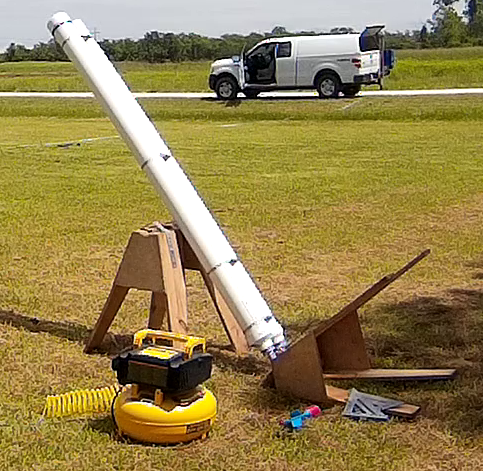
\includegraphics[width=\columnwidth]{PotatoCannon.png}}
 \caption{A pneumatic launcher for SeismicDarts.  Ballistic dart deployment has limited usefulness because the incident angle is equal to the firing angle.} 
 \label{fig:TradvsAutoDrop}
\end{figure}



\subsection{Simulation Studies}

A scheduling system to compare  time and costs for seismic surveys with varying numbers of UAVs, SeismicSpiders, SmartDarts, and Human manual laborers was coded in  {\sc Matlab}, available at \cite{Srikanth2016seismicScheduler}.

This tool allows us to examine engineering and logistic trade-offs quickly in simulation.  For example, Fig.~\ref{fig:DronevsTime} assumes a fixed number of darts, and examines the finishing time with $5$ to $500$ UAVs.  The time required decays asymptotically, but $140$ drones requires only twice the amount of time required for $500$ drones, indicating that $140$ are sufficient for the task. Lines are also plotted for $5000, 1000 and 500$ total darts.  In each case, substantial cost savings can be obtained by selecting the number of UAVs required to complete within $5\%$ of the optimal time.
The tool is useful for comparing the effectiveness of heterogeneous teams.  Table Fig.~\ref{fig:Sim_table} compares surveying a $1$ km x $10$ km strip of land with team (a) $5000$ seismic spiders(hexapods), (b) $500$ UAVs and $5000$ smart darts, (c) $500$ humans and $5000$ sensors(geophones).  Team (b) completed $6$ times faster than team (c).
In Fig.~\ref{fig:het_sen_ratio} we vary the percentage of individual type of sensor by keeping the total number of sensors a constant. The goal is to analyze ratios of different sensors to optimize cost and time. The number of drones employed for deploying smart darts is considered to be $10\%$ of number of smart darts available. We observe that employing UAVs brings down the deployment time. This is obvious since UAVs move at 20 m/s whereas SeismicSpiders move at 0.2 m/s. The drastic difference in velocities makes the UAV deployment time efficient. The SeimicSpiders are a special type of sensor that could be used for special cases like hard surface sensing or regions where it is difficult for UAvs to access like forests.

\begin{figure*}
\centering
\renewcommand{\figwid}{0.5\columnwidth}
\begin{overpic}[width =\figwid]{sim1_1.pdf}
\end{overpic}
\begin{overpic}[width =\figwid]{sim1_2.pdf}
\end{overpic}
\begin{overpic}[width =\figwid]{sim1_3.pdf}
\end{overpic}
\begin{overpic}[width =\figwid]{sim1_4.pdf}
\end{overpic}

\caption{Simulations were performed to estimate time take by different sensors a.) Only seismic spiders b.) Smart darts and deployment system c.) Heterogeneous System d.) Human workers
\label{fig:Sim_overview}}
\end{figure*}
\begin{figure} \centering
  {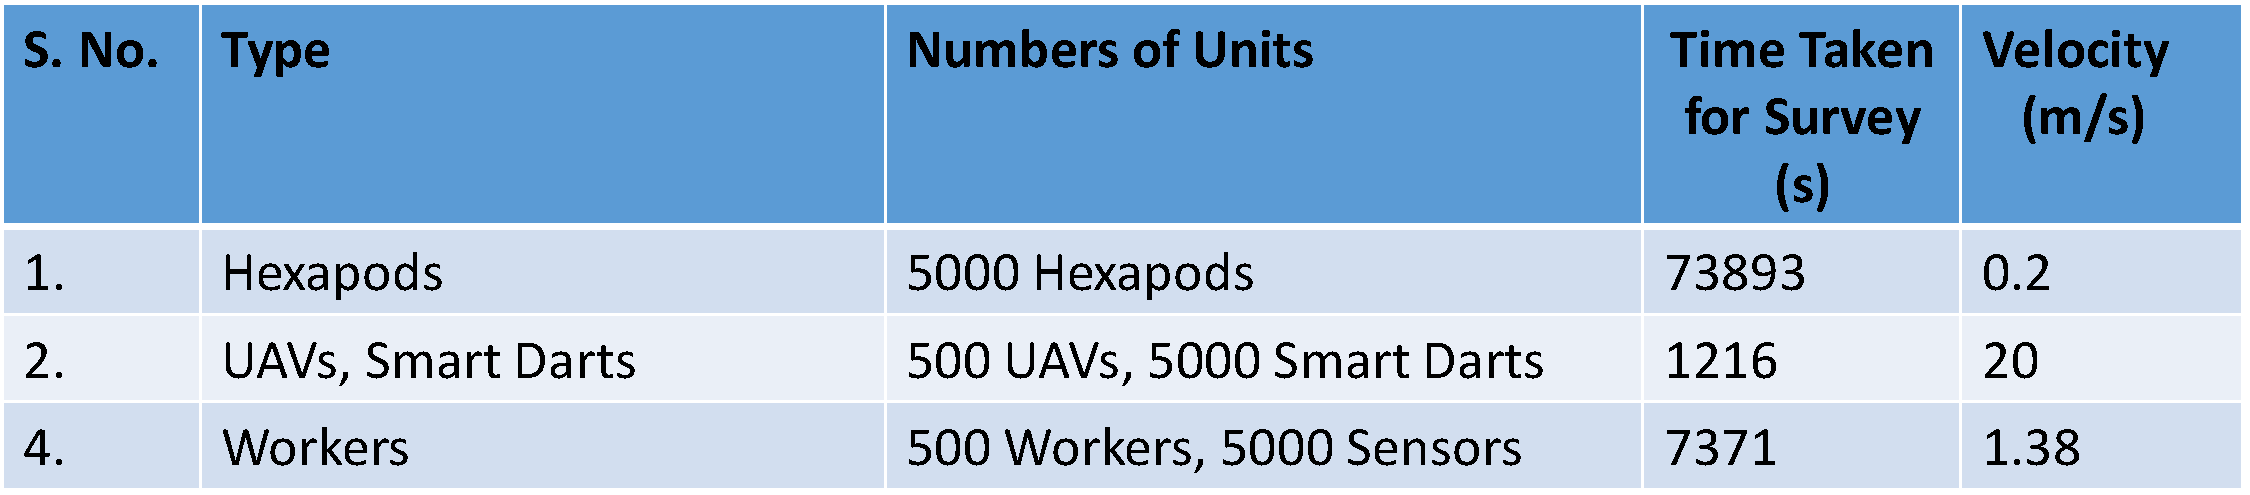
\includegraphics[width=\columnwidth]{simulation_table.pdf}}
 \caption{Comparison between different modes of deployment clearly indicate UAV deployment is highly efficient} 
 \label{fig:Sim_table}
\end{figure}
\begin{figure} \centering
  {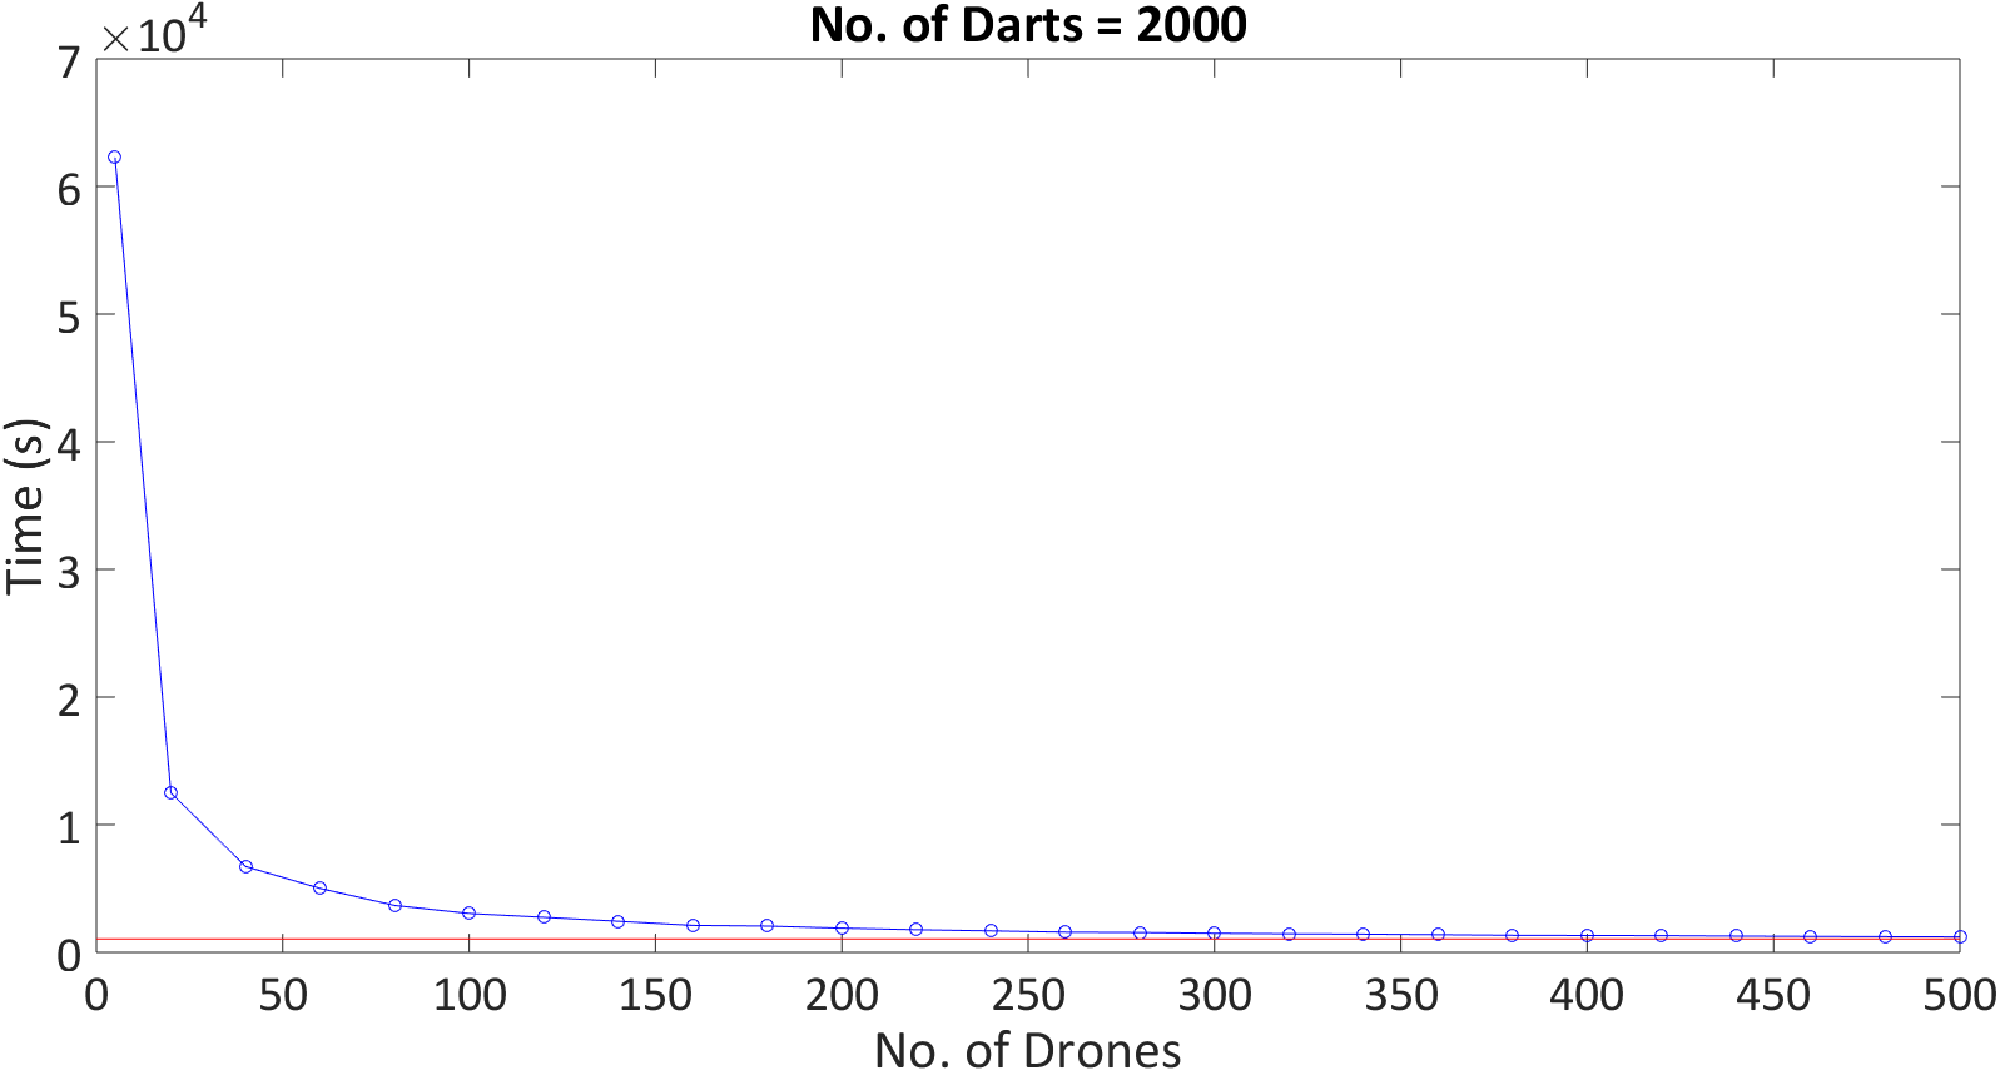
\includegraphics[width=\columnwidth]{DronevsTime.pdf}}
 \caption{This plot captures no. of drones vs time taken.} 
 \label{fig:DronevsTime}
\end{figure}
\begin{figure} \centering
  {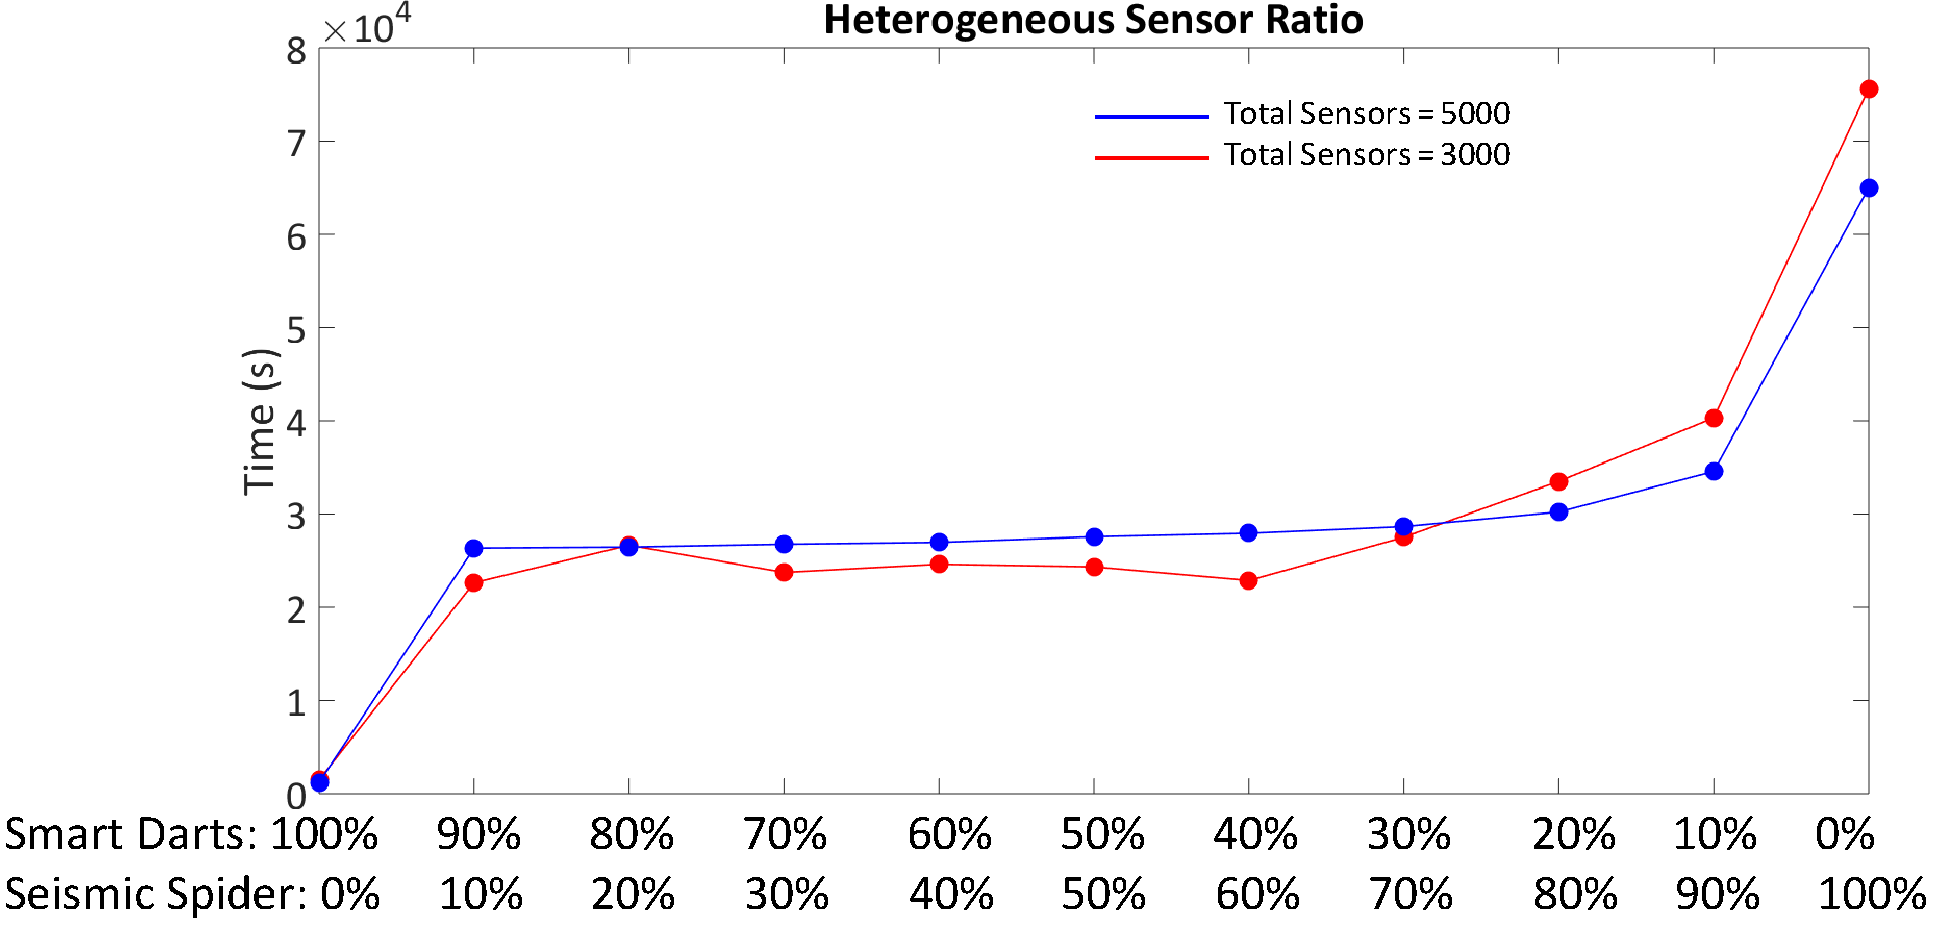
\includegraphics[width=\columnwidth]{het_sen_ratio.pdf}}
 \caption{This plot captures time with respect to different sensor ratios. The total number of sensors \{5000,3000\} were kept constant. UAVs were taken to be 10\% of darts for this experiment. } 
 \label{fig:het_sen_ratio}
\end{figure}